\documentclass{standalone}
\usepackage{tikz,amsmath}
\tikzset{ block/.style = {draw, fill=white, very thick, rectangle, minimum height=1cm, minimum width=2cm},}
\tikzset{sum/.style= {draw, fill=white, very thick, circle, node distance=1cm},}
\begin{document}
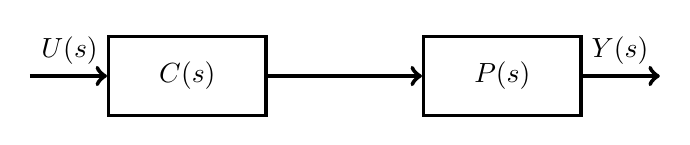
\begin{tikzpicture}[scale=2]
    \node[block](c)at(-0.5,0){$C(s)$};
    \node[block](p)at(1.5,0){$P(s)$};

    \draw[->,ultra thick](-1.5,0)node[above right]{$U(s)$}--(c.180);
    \draw[->,ultra thick](c.0)--(p.180);
    \draw[->,ultra thick](p.0)--(2.5,0)node[above left]{$Y(s)$};
\end{tikzpicture}
\end{document}